\begin{figure*}[!htbp]
\begin{minipage}{6in}
\begin{center}

\begin{minipage}{0.5\linewidth}
\begin{subfigure}[b]{\linewidth}
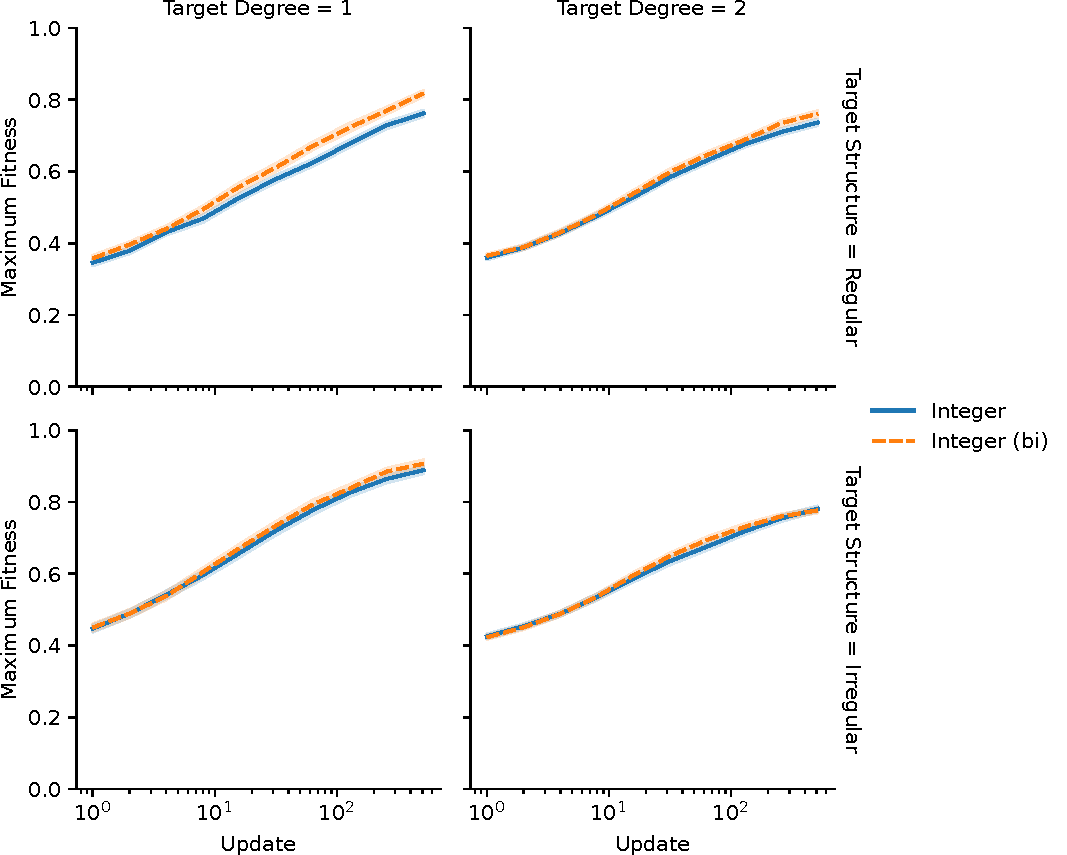
\includegraphics[width=\linewidth]{img/target_evolve_norm/viz=max-fitness-line+_data_hathash_hash=3e06b14c923ee265+_script_fullcat_hash=d2023baeff76b578+ext=.pdf}
\caption{Normally-distributed Mutation} \label{fig:norm_dist_mut}
\end{subfigure}
\end{minipage}%
\begin{minipage}{0.5\linewidth}
\begin{subfigure}[b]{\linewidth}
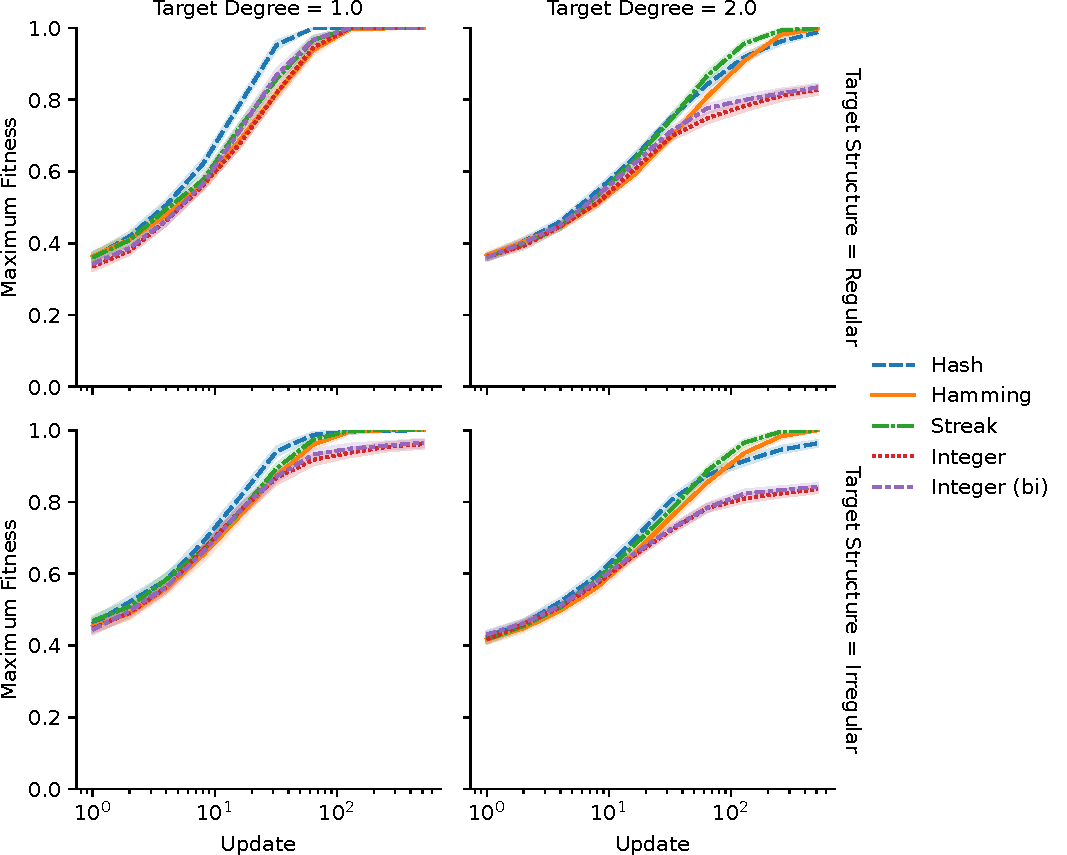
\includegraphics[width=\linewidth]{img/target_evolve/viz=max-fitness-line+_data_hathash_hash=4c78832f20b46ffd+_script_fullcat_hash=c26c8688c31571c2+ext=}
\caption{Bitwise mutation} \label{fig:bitwise_mut}
\end{subfigure}
\end{minipage}

\begin{minipage}{\linewidth}
\caption{
Trajectories of adaptive evolution for each tag-matching metric on the 32-vertex graph-matching task with normally-distributed mutation (\ref{fig:norm_dist_mut}) and bitwise mutation (\ref{fig:bitwise_mut}).
Maximum fitness is the best fitness value for any individual within a population.
Reported results use each metric's best-performing standard deviation mutation rate.
(See Supplementary Figure \ref{fig:evolve_norm_mutsweep} for survey showing how mutation rate affects adaptive evolution under each metric.)
Note log-scale x-axes.
Shaded area represents bootstrapped 95\% confidence intervals across 100 replicate observations.
}
\label{fig:evolve_bests_norm}
\end{minipage}
\end{center}
\end{minipage}
\end{figure*}
